\section{Background}
In this section we present the background of our research. We define our term and understanding of \textit{agent} and ABS and how we understand and use it in this paper, then we will give a description of the two kind of games which were the motivators for our research and case-studies and finally we will present related work.

\subsection{Agent-Based Simulation}
We understand ABS as a method of modelling and simulating a system where the global behaviour may be unknown but the behaviour and interactions of the parts making up the system is of knowledge. Those parts, called agents, are modelled and simulated out of which then the aggregate global behaviour of the whole system emerges. So the central aspect of ABS is the concept of an agent which can be understood as a metaphor for a pro-active unit, situated in a generic environment, able to spawn new agents and interacting with other agents in a network of neighbours by exchange of messages \cite{wooldridge_introduction_2009}. It is important to note that we focus our understanding of ABS on a very specific kind of agents where the focus is on communicating entities with individual, localized behaviour from out of which the global behaviour of the system emerges. We informally assume the following about our agents:

\begin{itemize}
	\item They are uniquely addressable entities with some internal state
	\item They can initiate actions on their own e.g. change their internal state, send messages, create new agents, kill themselves,...
	\item They can react to messages they receive with actions (see above)
	\item They can interact with a generic environment they are situated in
\end{itemize} 

An implementation of an ABS must solve two fundamental problems:

\begin{enumerate}
	\item \textbf{Source of pro-activity} How can an agent initiate actions without the external stimuli of messages?
	\item \textbf{Semantics of Messaging} When is a message \textit{m}, sent by agent \textit{A} to agent \textit{B}, visible and processed by \textit{B}?
\end{enumerate}

In computer systems, pro-activity, the ability to initiate actions on its own without external stimuli, is only possible when there is some internal stimulus, most naturally represented by some generic notion of monotonic increasing time-flow. Due to the discrete nature of computer-system, this time-flow must be discretized in steps as well and each step must be made available to the agent, acting as the internal stimulus. This allows the agent then to perceive time and become pro-active depending on time. So we can understand an ABS as a discrete time-simulation where time is broken down into continuous, real-valued or discrete natural-valued time-steps. Independent of the representation of the time-flow we have the two fundamental choices whether the time-flow is local to the agent or whether it is a system-global time-flow. Time-flows in computer-systems can only be created through threads of execution where there are two ways of feeding time-flow into an agent. Either it has its own thread-of-execution or the system creates the illusions of its own thread-of-execution by sharing the global one sequentially among the agents where an agent has to yield the execution back after it has executed its step. Note the similarity to an operating system with cooperative multitasking in the latter case and real multi-processing in the former.

\medskip 

The semantics of messaging define when sent messages are visible to the receivers and when the receivers process them. Message-processing could happen either immediately or delayed, depending on how message-delivery works. There are two ways of message-delivery: queued or immediate. In the case of immediate message-deliver the message is sent directly to the agent without any queuing in between e.g. a direct method-call. This would allow an agent to immediately react to this message as this call of the method transfers the thread-of-execution to the agent. This is not the case in the queued message-delivery where messages are posted to the message-box of an agent and the agent pro-actively processes the message-box at regular points in time.

\subsection{A discrete game: Prisoners Dilemma}
As an example of a discrete game we use the \textit{Prisoners Dilemma} as in \cite{nowak_evolutionary_1992}. In the prisoner dilemma two players play a game where in each step a player can either choose to cooperate or defect receiving a pay-off. There are four possible pay-offs: if both players cooperate both receive R; if one player defects and the other cooperates the defector receives T and the cooperator S; if both defect both receive P where T $>$ R $>$ P $>$ S.
In the version of \cite{nowak_evolutionary_1992} NxN agents are arranged on a 2D-grid where every agent has 8 neighbours. Agents don't have a memory of the past and have one of two roles: either cooperator or defector. In every step an agent plays the game with all its neighbours, including itself (something which was not explicitly mentioned in the paper but if omitted, will not lead to their results) and sums up the pay-off. After the pay-off sum is calculated the agent changes its role to the role of the agent with the highest pay-off within its neighbourhood (including itself). The authors attribute the following pay-offs: S=P=0, R=1, T$>$b, where b$>$1. They showed that when having a grid of only cooperators with a single defector at the center, the simulation will form beautiful structural patterns as shown in figure \ref{fig:sync_patterns}.

\begin{figure}
	\centering
	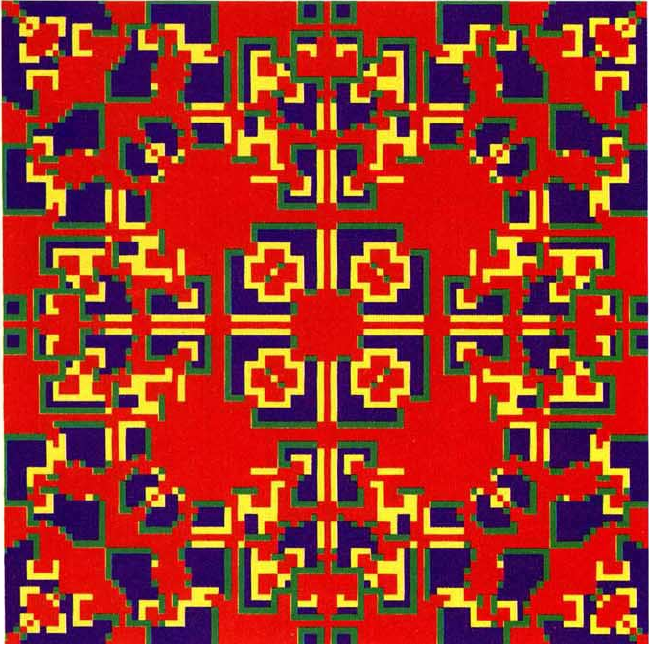
\includegraphics[width=.4\textwidth, angle=0]{./fig/sync_patterns.png}
	\caption{Patterns formed by playing the \textit{Prisoners Dilemma} game on a 99x99 grid with 1.8 $<$ b $<$ 2 after 217 steps. Blue are cooperators, red are defectors, yellow are cooperators which were defectors in the previous step, green are defectors which were cooperators in the previous step. Picture taken from \cite{nowak_evolutionary_1992}.}
	\label{fig:sync_patterns}
\end{figure}

In \cite{huberman_evolutionary_1993} the authors showed that the results of simulating the \textit{Prisoners Dilemma} as above depends on a a very specific strategy of iterating the simulation and show that the beautiful patterns seen in figure \ref{fig:sync_patterns} will not form when selecting a different update-strategy. They introduced the terms of synchronous and asynchronous updates and define synchronous to be as agents being updated in unison and asynchronous where one agent is updated and the others are held constant. Although the authors differentiated between the two strategies, their description still lacks precision and detail, something we will provide in this paper. Although they didn't publish their work in the field of ABS, it has general implications for ABS as well which can be generalized in the main message of our paper as emphasised in the introduction. We will show that there are more than two update-strategies and will give results of simulating this discrete game using all update-strategies.

\subsection{A continuous game: Heroes \& Cowards}
As an example for a continuous game we use the \textit{Heroes \& Cowards} game introduced by \cite{wilensky_introduction_2015}. In this game one starts with a crowd of agents where each agent is positioned randomly in a continuous 2D-space which is bounded by borders on all sides. Each of the agents then selects randomly one friend and one enemy (except itself) and decides with a given probability whether the agent acts in the role of a hero or a coward - friend, enemy and role don't change after the initial set-up. In each step the agent will move a small distance towards a target point. If the agent is in the role of a hero this target point will be the half-way distance between the agents friend and enemy - the agent tries to protect the friend from the enemy. If the agent is acting like a coward it will try to hide behind the friend also the half-way distance between the agents friend and enemy, just in the opposite direction. Note that this simulation is determined by the random starting positions, random friend and enemy selection, random role selection and number of agents. Note also that during the simulation-stepping no randomness is incurred and given the initial random set-up, the simulation-model is completely deterministic. As will be shown later the results of simulating this model are invariant under different update-strategies.

\begin{figure}
	\centering
	\includegraphics[width=.4\textwidth, angle=0]{./fig/heros_and_cowards.png}
	\caption{A conceptual diagram of the \textit{Heroes \& Cowards} game. Hero (green) and coward (red) have the same agents as friend and enemy but act different: the hero tries to move in between the friend and enemy whereas the coward tries to hide behind its friend.}
	\label{fig:heros_and_cowards}
\end{figure}

\subsection{Related Research}
\cite{a_framework_2008} give an approach for ABS on GPUs which is a very different approach to updating and iterating agents in ABS. They discuss execution order at length, highlight the problem of inducing a specific execution-order in a model which is problematic for parallel execution and give solutions how to circumvent these shortcomings. Although we haven't mapped our ideas to GPUs we explicitly include an approach for data-parallelism which, we hypothesize, can be utilized to roughly map their approach onto our terminology. 
	
\medskip
	
\cite{botta_time_2010} sketch a minimal ABS implementation in Haskell which is very similar in the basic structure of ours. This proves that our approach seems to be a very natural one to apply to Haskell. Their focus is primarily on economic simulations and instead of iterating a simulation with a global time, their focus is on how to synchronize agents which have internal, local transition times. Although their work uses Haskell as well, our focus is very different from theirs and approaches ABS in a more general and comprehensive way.

\medskip

\cite{dawson_opening_2014} describe basic inner workings of ABS environments and compare their implementation in C++ to the existing ABS environment AnyLogic which is programmed in Java. They explicitly mention asynchronous and synchronous time-models and compare them in theory but unfortunately couldn't report the results of asynchronous updates due to limited space. They interpret asynchronous time-models to be the ones in which an agent acts at random time intervals and synchronous time-models where agents are updated all in same time intervals.

\medskip

\cite{yuxuan_agent-based_2016} presents a comprehensive discussion on how to implement an ABS for state-charts in Java and also mentions synchronous and asynchronous time-models. He identifies the asynchronous time-model to be one in which updates are triggered by the exchange of messages and the synchronous ones which trigger changes immediately without the indirection of messages.

\medskip

\cite{jankovic_functional_2007} discuss using functional programming for discrete event simulation (DES) and mention the paradigm of Functional Reactive Programming (FRP) to be very suitable to DES. We were aware of the existence of this paradigm and have experimented with it using the library Yampa, but decided to leave that topic to a side and really keep our implementation clear and very basic.

\medskip

The amount of research on using Haskell in the field of ABS has so far been moderate. Though there exist a few papers which look into Haskell and ABS \cite{de_jong_suitability_2014}, \cite{sulzmann_specifying_2007}, \cite{jankovic_functional_2007} they focus primarily on how to specify agents. An library for Discrete Event Simulation (DES) and System Dynamics (SD) in Haskell called \textit{Aivika 3} is described in \cite{sorokin_aivika_2015}. It also comes with very basic features for ABS but only allows to specify simple state-based agents with timed transitions. This papers is investigating Haskell in a different way by looking into its suitability in implementing update-strategies in ABS, something not looked at in the ABS community which presents an original novelty as well.

\medskip

There already exists research using the Actor Model for ABS in the context of Erlang \cite{varela_modelling_2004}, \cite{di_stefano_using_2005}, \cite{di_stefano_exat:_2007}, \cite{sher_agent-based_2013} but we feel that they barely scratched the surface. We want to renew the interest in this direction of research by incorporating Scala with using the Actor-library in our research because we will show that one update-strategy maps exactly to the Actor Model.